Seit der Entdeckung von Victor Hess der kosmischen Höhenstrahlung
1912 feiert die Astroteilchenphysik bahnbrechende errungenschaften.
Die Entdeckung der kosmischen Hintergrundstrahlung gilt als beleg des
expandierendes Universum und wirft dennoch weitere Fragen zum frühen Universum auf.
Die Kosmische Strahlung lässt das erforschen elementarer Bausteine und
Beschlunigungsprozesse zu wovon
einige informationen über ihren Usprung tragen.
Anhand der kosmischen Botenteilchen wozu neuerdings aus Graviatationswellen
zählen werden Informationen über supernovae, schwarze löcher extrahiert.
\section*{MAGIC}%
\label{sec:magic}
\begin{wrapfigure}[13]{o}{0.45\textwidth}
		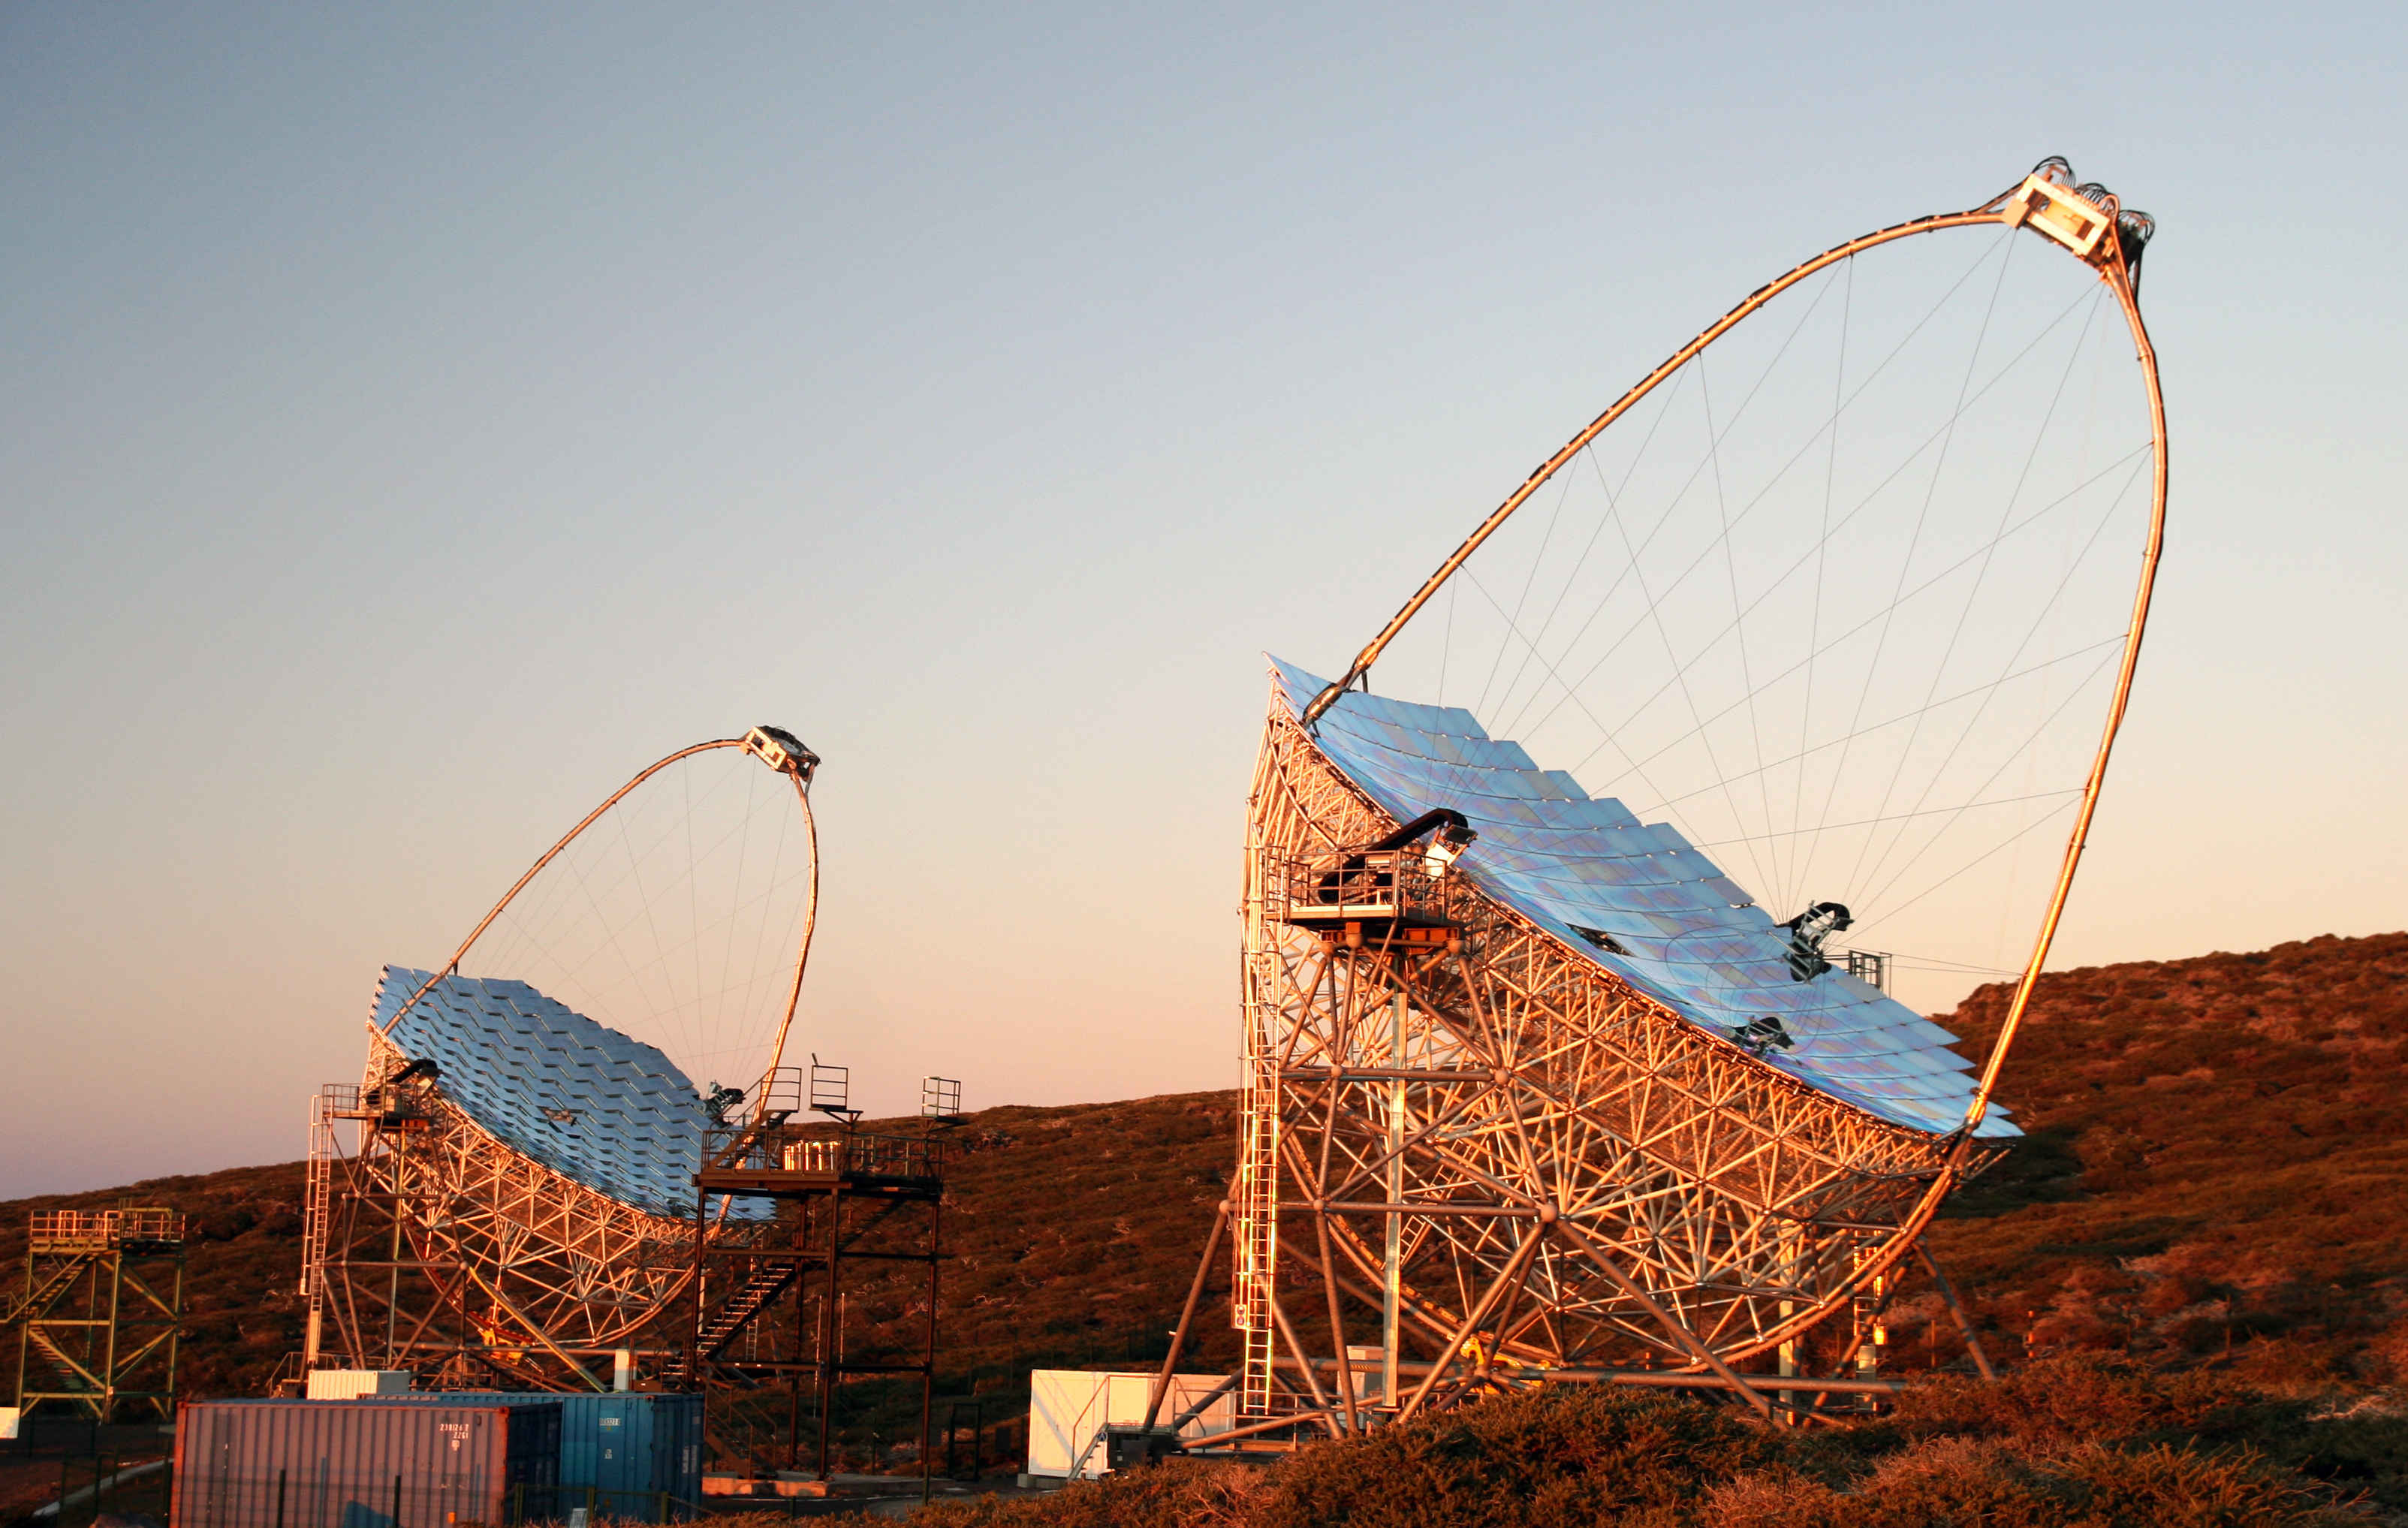
\includegraphics[width=\linewidth]{pictures/magic.JPG}
		\caption{Magic Teleskope in Observationsstellung.}%
		\label{fig:magic}
\end{wrapfigure}
Der Nachweis von hochenergetischer Gammastrahlung ist auf der Erde aufgrund der
Atmosphäre nur indirekt möglich.
Hochenergetisches Teilchen erzeugen in der Atmosphäre Teilchenschauer, die
aufgrund ihrer relativistischen Geschwindigkeite Tscherenkovlicht abstrahlen.
Magic ist derzeit (16.11.2016) das größte Stereoteleskop mit dem die
Detektion von Tscherenkov-Schauern in einem Energiebereich von
\SI{50}{\giga\electronvolt} bis \SI{50}{\giga\electronvolt} möglich ist.
Es steht auf der Insel La Palma auf einer Höhe von \SI{2200}{\meter}.
Trifft ein Teilchen mit Überlichtgeschwindigkeit in einem Medium, so emittiert
dieses einen Tscherenkov-Kegel.
Die ultrarelativistischen Teilchen welche auf die Erdatmosphäre treffen
Wechselwirken mit den darin enthaltenen Teilchen beispielsweise über
Bremsstrahlung, Paarerzeugung \ldots und produzieren somit weitere
relativistische Teilchen welche wiederum Tscherenkov kegel erzeugen.

Die dadurch erzeugten Lichtblitze können durch Tscherenkov-Teleskope detektiert
werden.
Die Spiegelfläche von \SI{17}{\meter} Durchmesser besteht aus \num{974} einzelnen
Spiegeln die auf \num{1039} Photo Multiplier Tubes (PMTs) mit einem
Field of View von \SI{3.5}{\degree} abbilden.

Ziel ist es mit den Teleskopen Gamma-Quellen wie AGNs, Supernovae und
Gasverteilungen in denen viel Sternbildung stattfindet genauer zu observieren.
Desweiteren wird nach einen indirekten Nachweis nach dunkeler Materie
Fundamentales Problem geladenen Teilchen jegliche Richtungsinformation verlieren
in kosmologischen Magnetfelder verlieren und somit keine Informationen aus
Quelle rekonstruiert werden.

\section*{Krebsnebel}%
\label{sec:krebsnebel}

In diesem Versuch wird der Krebsnebel untersucht. 
Er ist eine Überrrest einer Supernova-Explosion eines Sterns,
mit 8~bis 12 Sonnenmassen aus dem Jahre 1054 
und befindet sich im Sternbild Stier.
\begin{wrapfigure}[16]{L}{0.35\textwidth}
		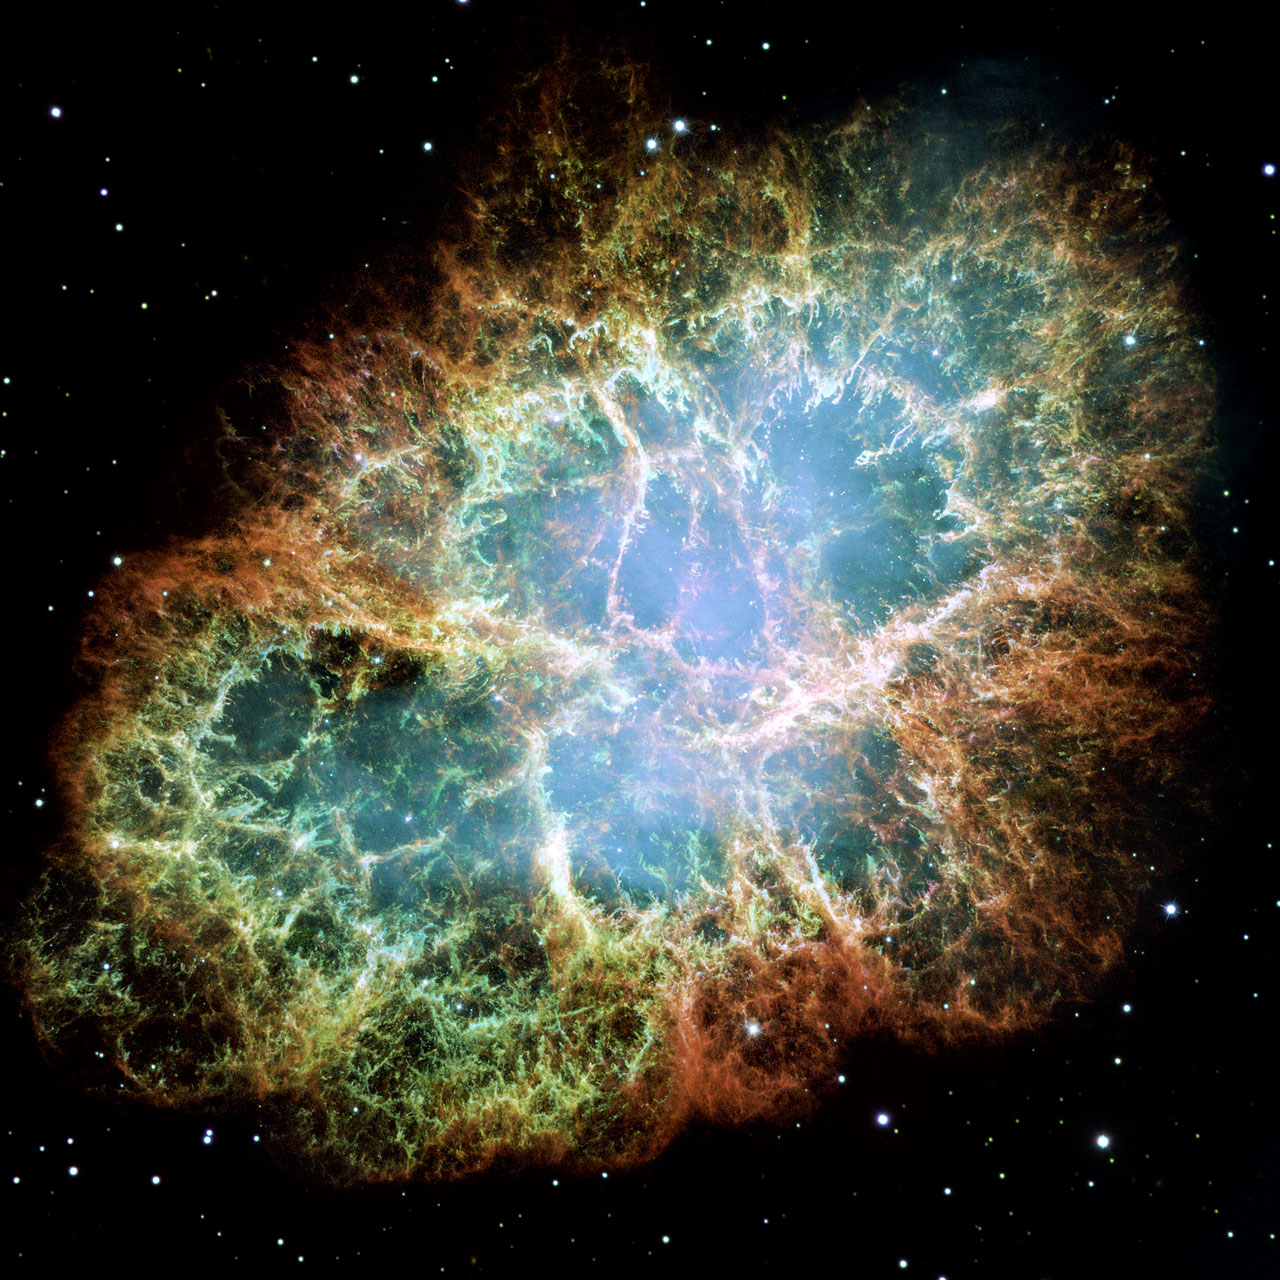
\includegraphics[width=\linewidth]{pictures/crab.jpg}
		\caption{Krebsnebel aufgenommen mit dem Hubble Teleskop.}%
		\label{fig:magic}
\end{wrapfigure}

Eine Supernova-Explosionen ist das Ende eines Massereichen Sterns, 
welcher jedoch nicht schwer genug,
für die Bildung eines schwarzen Loches ist.

Im Zentrum befindet sich ein Pulsar welcher die Quelle von starker
elektromagnetischer Strahlung ist.
Pulsare sind schnell rotierende Neutronensterne,
welche ein sehr regelmäßiges und kurzes Pulse emittieren.
Typische größen von Neutronensterne sind Durchmesser von einigen
\SI{10}{\kilo\meter}.
Die Materiereste die bei einer Supernova-Explosion,
vom zurückbleibenden Neutronenstern abgesprengt werden,
bilden eine Astronomisches Objekt,
welches sich in Astronomischen Zeitskalen schnell verändert.

Der Krebsnebel kann in Allen Kanälen von der Radio bis hin zur Gamma-Ray
Astronomie observiert werden.
Aufgrund seiner Eigenschaften wird er als Standardkerze der Astronomie betitelt,
da die Eigenschaften sehr gut bekannt sind und sich die performance von
Teleskopen verglichen werden kann. 
\clearpage
